\setchapterimage[7cm]{ztf/ztf_telescope.png}
\chapter{The Nuclear Sample}\label{ztf}
\labch{nucsam}
Motivated by the three neutrinos coincident with accretion phenomena in the cores of active galaxies, it will be instructive to create a systematic sample of nuclear transients in the ZTF footprint. Furthermore, with the advent of a deep high-cadence sky surveys in the form of the Legacy Survey of Space and Time (LSST, hosted by the Vera C. Rubin Observatory)~\sidecite{Ivezic2019} in the near future, photometric identification of transients will be crucial.

The rate of transients detected by LSST will by far exhaust the available spectroscopic resources, thus requiring informed decisions about when to rely on spectroscopy for classification and characterization. The vast majority of LSST-detected transients will either be photometrically classified, or not classified at all. Therefore, photometrically classifying the ZTF nuclear transients can serve as a precursor study to LSST-era astronomy.

This chapter is dedicate to the nuclear sample, and is structured as follows: A discussion on the sample creation will be followed by different methods to classify the sample. This will be done with a special focus on TDEs.

\section{Sample Creation}
The nuclear sample was created with \texttt{AMPEL} (see Section~\ref{ampel}), using its capability to rerun analyses on archival data. To perform such a rerun, a modified version of the \texttt{AMPEL} nuclear filter was used.

\subsection{\texttt{AMPEL} Nuclear Filter}
\begin{marginfigure}
    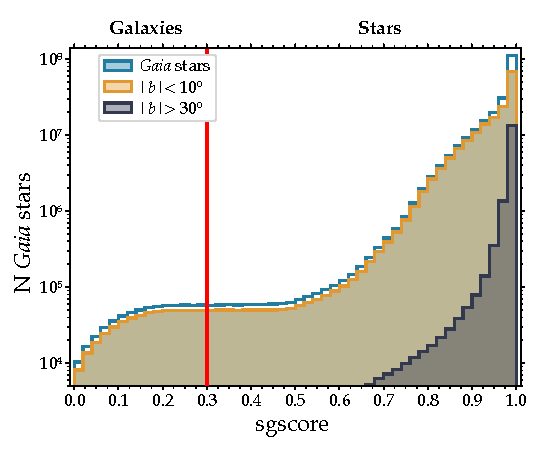
\includegraphics{nuclear/sgscore.pdf}
    \caption[\texttt{sgscore} performance]{\texttt{sgscore} performance evaluated with known \textit{Gaia} stars. At the chosen threshold of 0.3 (red line), the misidentification of stars as galaxies is negligible. Adapted from~\cite{Tachibana2018}}
    \labfig{sgscore}
\end{marginfigure}
The filter is used primarily by the ZTF TDE working group to scan for transient activity that is compatible with an emerging TDE~\cite{Velzen2021a}. In the rerun, it was slightly modified, and used to evaluate each and every alert issued by ZTF.

The logic behind the filtering process can be explained as follows: It selects events with a minimum of photometric quality, ensured by minimum requirements on the number of detections and the brightness. The event at least once needs to pass as `real' (opposed to bogus), and the host needs a high probability of passing as galaxy, not star. Furthermore, \textit{Gaia} is consulted to veto against stars, and the events need to be nuclear, i.e. happen close to the core of their host galaxy.

The criteria used were:
\begin{description}
    \item[\texttt{sgscore}] As detailed in Section~\ref{ztf_image_subtraction}, \texttt{sgscore} is a machine-learning based star-galaxy score for PS1 objects (low values: galaxy, high values: stars). The transient must at least once have an \texttt{sgsscore} < 0.3 to pass the filter.
    \item[Number of detections] At least 3 detections in both ZTF \textit{g}- and \textit{r}-band are required.
    \item[Galactic cut] The object must be separated by at least \SI{5}{\degree} from the galactic plane to avoid contamination by foreground stars.
    \item[PS1 photometry] To avoid crowded areas, transients where more than 100 objects in the vicinity have a counterpart in PS1 are removed.
    \item[Brightness] At least one alert datapoint of the transient must be brighter than 20 mag.
    \item[\texttt{rbscore}] The real-bogus score separating erroneous detections (low values) from real ones (high values, see Section~\ref{ztf_alerts}) must be larger than 0.3. Note that for more recent data, also \texttt{deep real bogus} is available, which promises vastly better results \sidecite{Duev2019}. Older alerts from 2018 or 2019 do not contain this information, and there is no direct translation from an \texttt{rbscore} threshold to a \texttt{drbscore} threshold. For these reasons and to maximize consistency, we restricted ourselves to using only the older \texttt{rbscore}. The quite loose cut of 0.3 does not entail overly large contamination, as we also require the transient to have a PS1 counterpart. Figure~\ref{fig:rbvsdrb} shows a comparison of the False Negative Rate (FNR) of \texttt{rbscore} vs. \texttt{drbscore}. At the chosen threshold of $0.3$, the FNR for both algorithms is a the percent level.
    \item[Core distance] For all objects that make it this far, their distance to the core is computed. To make this more robust, three different distance metrics are computed. The \textbf{mean distance} to the PS1 source in the reference images, the \textbf{median distance} to that, and lastly, a \textbf{weighted distance}. The latter is computed according to~\sidecite{Velzen2019} and accounts for the fact that the RMS of the angular core distance scales linearly with magnitude. $\sigma_\text{dist}$ = $0.24 + 0.04(m-20)$, where $m$ is the difference photometry magnitude. This stage rejects all transients for which none of the three distances lies below 0.5 arcseconds.
\end{description}

\begin{figure}[htpb]
    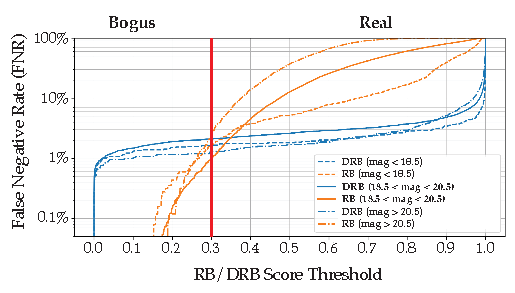
\includegraphics[width=0.9\textwidth]{nuclear/rb_v_drb.pdf}
    \caption[\texttt{rbscore}/\texttt{drbscore} performance]{\texttt{rbscore} vs \texttt{drbscore} performance, evaluated in terms of false negative rate as a function of the threshold. Adapted from~\cite{Duev2019}. The chosen threshold of 0.3 is shown as red vertical line. At that value, \texttt{rbscore} has a False Negative Rate of \SI{\approx1}{\percent} in the relevant magnitude range of $18.5 < \text{mag} < 20.5$.}
    \labfig{rbvsdrb}
\end{figure}

This filter was then applied to all ZTF alerts issued between 1 July, 2018 and 1 January, 2022, comprising 3.5 years of data in total.

\subsection{Rejection Statistics}
From a total sample of XXX alerts issued by ZTF during these 3.5 years, ultimately \textcolor{red}{11687} nuclear transients are selected. The survival rates during the filtering process are shown in Fig.~\ref{fig:nuclear_decision}.

\begin{figure}[htpb]
    \begin{tikzpicture}[node distance=1.2cm]
        \node (start) [keep] {XXX initial ZTF alerts};
        \node (dec1) [decision,  font=\small, align=center, below of=start] {SQL\\Filter};
        \node (expl1) [explain, font=\small, align=left, left of=dec1, xshift=-1.8cm] {$<20$ mag\\\texttt{rbscore} $>0.3$\\PS1 dist $<0.5$ arcsec\\$\geq 3$ detections};
        \node (disc1) [discard, font=\small, right of=dec1, xshift=2.1cm] {Discard xx alerts};
        \node (keep1) [keep, font=\small, below of=dec1] {Keep 94,714,866 alerts};
        \node (dec2) [decision, font=\small, align=center, below of=keep1] {\texttt{sgscore}\\veto};
        \node (expl2) [explain, font=\small, align=left, left of=dec2, xshift=-2.2cm] {\texttt{sgscore} $\leq0.3$};
        \node (disc2) [discard, font=\small, right of=dec2, xshift=2.3cm] {Discard 94,485,886 alerts};
        \node (keep2) [keep, font=\small, below of=dec2] {Keep xx alerts};
        \node (dec3) [decision, font=\small, align=center, below of=keep2] {PS1\\veto};
        \node (expl3) [explain, font=\small, align=left, left of=dec3, xshift=-1.5cm] {PS1 source faint enough\\good PS1 photometry};
        \node (disc3) [discard, font=\small, right of=dec3, xshift=2cm] {Discard xx alerts};
        \node (keep3) [keep, font=\small, below of=dec3] {Keep xx alerts};
        \node (dec4) [decision, font=\small, align=center, below of=keep3] {Photometry\\veto};
        \node (expl4) [explain, font=\small, align=left, left of=dec4, xshift=-1.5cm] {$<20$ mag\\$\geq$ 3 detections\\flux increase $>2.5$ mag};
        \node (disc4) [discard, font=\small, right of=dec4, xshift=2cm] {Discard xx alerts};
        \node (keep4) [keep, font=\small, below of=dec4] {Keep xx alerts};
        \node (dec5) [decision, font=\small, align=center, below of=keep4] {Position\\veto};
        \node (expl5) [explain, font=\small, align=left, left of=dec5, xshift=-1.5cm] {$>5$ deg from gal. plane\\not potential mover};
        \node (disc5) [discard, font=\small, right of=dec5, xshift=2cm] {Discard xx alerts};
        \node (keep5) [keep, font=\small, below of=dec5] {Keep xx alerts};
        \node (dec6) [decision, font=\small, align=center, below of=keep5] {\textit{Gaia}\\veto};
        \node (expl6) [explain, font=\small, align=left, left of=dec6, xshift=-1.5cm] {No match to \textit{Gaia} star\\$\leq30$ \textit{Gaia} stars close by};
        \node (disc6) [discard, font=\small, right of=dec6, xshift=2cm] {Discard xx alerts};
        \node (keep6) [keep, font=\small, below of=dec6] {Keep xx alerts};
        \draw [arrow] (start) -- (dec1);
        \draw [arrow] (keep1) -- (dec2);
        \draw [arrow] (dec1) -- node[midway,above] {\small no} (disc1);
        \draw [arrow] (dec1) -- node[midway,left] {\small yes} (keep1);
        \draw [arrow] (dec2) -- node[midway,above] {\small no} (disc2);
        \draw [arrow] (dec2) -- node[midway,left] {\small yes} (keep2);
        \draw [arrow] (keep2) -- (dec3);
        \draw [arrow] (dec3) -- node[midway,above] {\small no} (disc3);
        \draw [arrow] (dec3) -- node[midway,left] {\small yes} (keep3);
        \draw [arrow] (keep3) -- (dec4);
        \draw [arrow] (dec4) -- node[midway,above] {\small no} (disc4);
        \draw [arrow] (dec4) -- node[midway,left] {\small yes} (keep4);
        \draw [arrow] (keep4) -- (dec5);
        \draw [arrow] (dec5) -- node[midway,above] {\small no} (disc5);
        \draw [arrow] (dec5) -- node[midway,left] {\small yes} (keep5);
        \draw [arrow] (keep5) -- (dec6);
        \draw [arrow] (dec6) -- node[midway,above] {\small no} (disc6);
        \draw [arrow] (dec6) -- node[midway,left] {\small yes} (keep6);
    \end{tikzpicture}
    \caption[Nuclear filter flow chart]{Flow chart showing the workings of the nuclear filter.}
    \labfig{nuclear_decision}
\end{figure}

As one can see, the vast majority of alerts are rejected based on them being either too faint, likely being bogus, or likely being stars.

\subsection{Forced photometry}
To be sensitive to early and late-time light curve evolution, forced photometry was acquired for all 11687 transients making the final cut. This was again done with \texttt{fpbot}, see Section \ref{fpbot} for details. The process proved cumbersome due to the enormous data volume (several hunders of GB) that was required to be transferred from IPAC and stored in batches due to computing center restrictions.

\subsection{Infrared Data}
Motivated by the strong dust echo detected for AT2019dsg, AT2019fdr and AT2019aalc, the optical forced photometry dataset was completed with infrared light curves from the \textit{WISE} mission. This was achieved by using the \texttt{timewise} package~\sidecite{Necker2023a} to download all datapoints available for each source location in the \textit{W1}- and \textit{W2}-band.

Most sources have infrared counterparts, sampled with a half-year cadence in both bands.

\subsection{Catalog Matching}
To enrich the sample by information available on the transients, these were crossmatched to a variety of catalogs and services. These comprised:

\begin{description}
    \item[Spectroscopic Redshifts] To obtain \textbf{spectroscopic redshifts}, the \texttt{AMPEL} module \texttt{T2DigestRedshifts} was employed. This queries the following services: A local database of the spectroscopic redshifts contained in the NASA/IPAC Extragalactic Database (NED)\sidenote{\url{https://ned.ipac.caltech.edu}}, spectroscopic redshifts from SDSS, and finally redshifts from the Galaxy List for the Advanced Detector Era (GLADE)~\sidecite{Dalya2018} v2.3.
    \item[Photometric Redshifts] Additionally, \texttt{T2DigestRedshifts} also provides \textbf{photometric redshifts} from the Legacy Survey~\sidecite{Zhou2020}, the 2MASS Photometric Redshift Catalog~\sidecite{Bilicki2013}, and photometric redshifts from the PS1 Source Types and Redshifts with Machine learning (PS1-STRM) catalog~\sidecite{Beck2020}.
    \item[Marshal/Fritz] During ZTF Phase I, the GROWTH Marshal~\sidecite{Kasliwal2019} served as a community hub to gather information on single transients. This service has been replaced by Fritz~\sidecite{Coughlin2023} with the same design goal. Both were queried for transient classifications.
    \item[TNS] The Transient Name Server (see Section~\ref{catmatch}) was also used to obtain classifications and redshifts of known transients.
    \item[AllWISE] Additionally to the \textit{WISE} light curves, archival data from the first part of the \textit{WISE} mission was obtained. This had the advantage of providing two more bands (\textit{W3} and \textit{W4}), which allowed for the calculation of more colors. This was used in AGN rejection, see \textcolor{red}{Section}.
    \item[CRTS DR1] The Catalina Real-time Transient Survey Catalog contains cataclysmic variables which are crossmatched against to reduce contamination by foreground stars.
    \item[SDSS] The Sloan Digital Sky Survey is also used to crossmatch against foreground stars.
\end{description}

\section{Light Curve Fits}
To classify the transients, the following strategy was employed: Fit all transients with a dedicated TDE light curve model, as well as a supernova Ia model. Both fit results can then be employed in feature-extraction based machine learning algorithms.

\subsection{TDE Model Fit}

\subsection{SNIa Fit}
As \textbf{SNe Ia are a prominent contaminant} for bona fide nuclear events (i.e.~such events that can only occur in the centers of galaxies), it is crucial to identify them. To achieve this goal, all light curves were subjected to a fit using the tried and tested Spectral Adaptive Lightcurve Template (SALT2)~\sidecite{Guy2007} light curve model.

SALT2 assumes the light curve is indeed a supernova Ia and applies empirical corrections to the light curve color and stretch (i.e.~the width of the light curve). This is achieved by matching templates generated by a set of well-sampled Ia light curves and spectra of varying distance. The resulting color and stretch correction parameters, as well as the peak brightness and the reduced $\chi^2$ were saved and will later be used as features in training a machine learning model.

\begin{figure}[htb]
    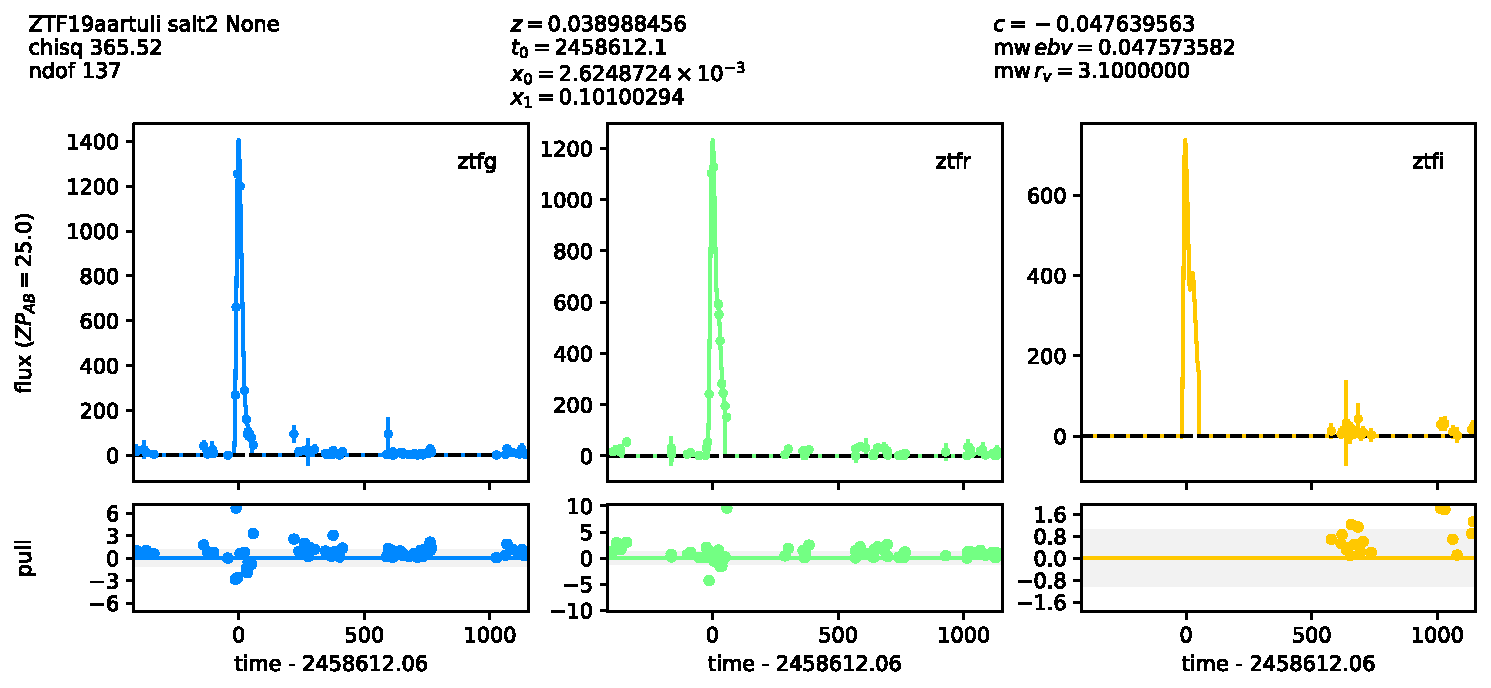
\includegraphics[width=1\textwidth]{nuclear/salt.pdf}
    \caption[SALT2 Fit]{Examplary SALT2 fit output. The three panels show three ZTF bands. Time 0 is the fitted peak of the assumed SN Ia; and as one can see the transient in question is fairly well approximated by SN Ia light curve, with a reduced  $\chi^2=2.67$. The transient is in a fact a spectroscopically classified supernova Ia.}
    \labfig{salt2}
\end{figure}